\documentclass[sigconf]{acmart}

\settopmatter{printacmref=false}
\makeatletter
\setcopyright{none}
\renewcommand\footnotetextcopyrightpermission[1]{}
\makeatother
\pagestyle{plain}

\usepackage{booktabs} 


\begin{document}

\title{Report Foundations of Data Science Group Project}


\begin{abstract}

When we collect data from the real world, they often contain errors, omissions, or inconsistencies that would be better to correct before analyzing it.

\end{abstract}

\maketitle

\section{Cleaning data}

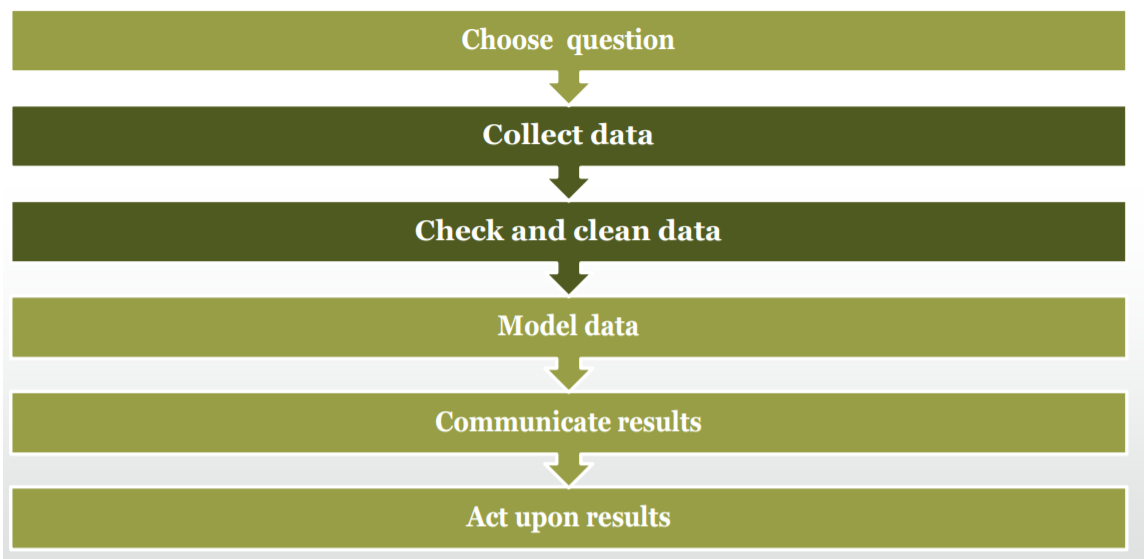
\includegraphics[width=0.40\textwidth]{aa.png}

\subsection{First step : Download } 
For this group project we collected data from the website oanda.com . These data were about weekly average exchange rates from December 1998 to December 2017. We considered all currency of the G20's countries and we downloaded all data considering the GBP as base currency. Every file downloaded was made in this way : 

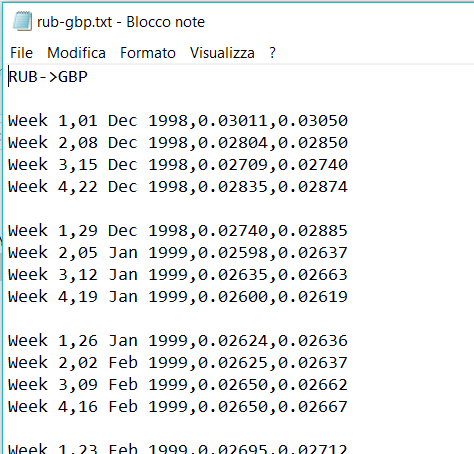
\includegraphics[width=0.25\textwidth]{aaa2.png}


\begin{itemize} 
\item Size of table : 1240 x 4 columns 
\item Col[0]= Week(1,2,3,4) 
\item Col[1]= Month-Year(i.e may 2002) 
\item Col[2]= Bid ( Bid is the price a buyer is willing to pay for a security) 
\item Col[3]= Ask ( Ask is the price a seller is willing to accept for a security) 
\end{itemize}

I had 16 files(are 16 because in the G20 group there is France Italy and Germany where the currency is Euro and also there is one member called European union that is a representative of UE) and I wrote, using a python, a script called CLEANING.PY that i used to clean my data. I gave in input a file formed by 1240(included blank space between rows) x 4 columns and i received in output something like this : 

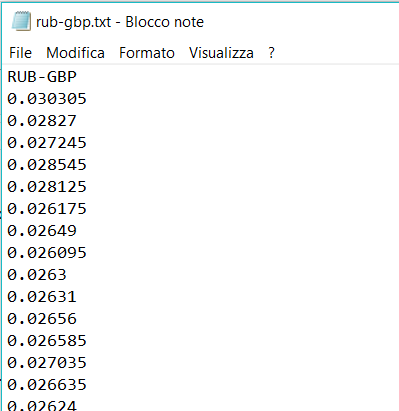
\includegraphics[width=0.25\textwidth]{aaa1.png}

Using my python script I removed all spaces, the time that i saved in one different file, and I calculated an average between bid and ask.

\subsection{Third step : Creation of a complete matrix } 
I wrote another py script called completeMatrix.py that i used to create all possible currency pair. Remembering that the currency were 16 , I had in output a matrix with 16x16 column and 994 rows.
 

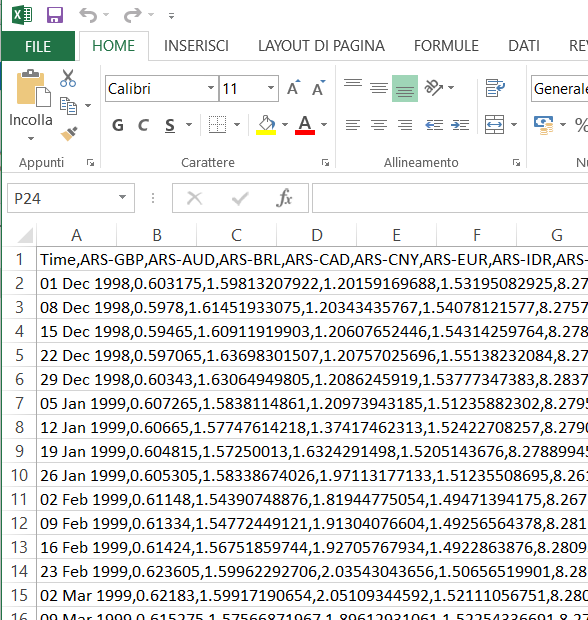
\includegraphics[width=0.4\textwidth]{bbb.png}


\section{Model Data}

\subsection{Purpose}

The target for this assignment was to find, giving in input one currency exchange, the \textbf{three} most relevant currency exchanges that influence the most the input. To do that we consider the matrix containing all possible combinations of currency exchanges and we used the software Matlab. We used the technique of regression to create a model that eventually in the will predict future values of currency exchange, and we calculated the "relevant variables", that are those variables that influence the input the most 

\subsection{Procedure}
\subsubsection{Find the 3 most relevant variable \\}

To find the most relevant exchange rates for the input, it was necessary to write a Matlab script where it was used the CVX tool. CVX is a modeling system for constructing and solving disciplined convex programs (DCPs). {\cite{1}}

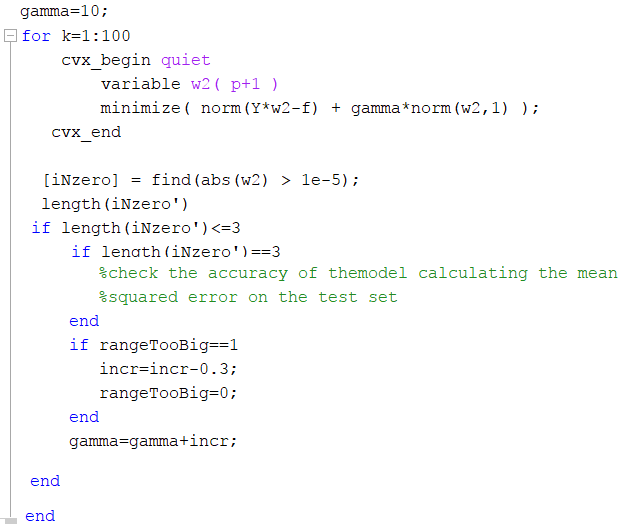
\includegraphics[width=0.4\textwidth]{ccc.png}

Explanation of the procedure : 

\begin{itemize}
\item cvx\_begin : must be written as the first instruction of a CVX model
\item cvx\_begin quiet : prevents the model from producing any screen output while it is being solved.
\item cvx\_end : must be the last instruction of the CVX procedure 
\item variable : it is used to declare the variable, it includes the name
of the variable, an optional dimension list, and one or more keywords that provide additional information about the content or structure of the variable.
\item minimize : it is a command used to declare an objective function( can be also maximize) 
N.B. The objective function in a call to minimize must be convex; the objective function in a call to maximize must be concave. In this case Y*w2-f is convex.
\textbf{Goal : find the best weights vector that minimize the error }
\item +gamma(w2) : I used gamma for the ℓ1 regularization like \textit{\textbf{Lasso}}. This technique is normally used to solve the overfitting problem in statistical models. \textbf{In this particular case we thought that it was a good idea because we built a model using 211 different variables and so the model was complex and the risk of overfitting was high}
\item find(abs(w2)\textgreater(1e-5) : we found which wights are not switched off by the regularizer, that are the most relevant variables. 
\end{itemize}

After obtained the most relevant values, we split all the data in training set and test set and  we calculated the MSE (means squared error) on the test set. After executed 15 times the script I had, on average, an error of 20 on the test set. 


\subsubsection{Justification about gamma \\}

One of the most difficult thing was about setting gamma for the regularization. After made some research we understood that it is almost impossible set a good gamma because it is totally dependent on both the training set and all parameters that were used\cite{2}. 

\begin{itemize}
\item Gamma is dependent on both the training set and the other parameters you use.
\item There is no “good Gamma” for any data set alone
\item Mathematically you call “Gamma” the “Lagrangian multiplier” (complexity control).
\item The higher Gamma is, the higher the regularization. Increasing lambda results in less overfitting but also greater bias.
\item Gamma values around 20 are extremely high, and should be used only when you are using high depth or if you want to control the directly the features which are dominating in the data set (i.e too strong feature engineering). 

\end{itemize}

To find the most relevant values, based on the dataset, gamma was changed automatically in every iteration, and so it was increased until exactly three variables were not switched off.

\subsubsection{Create a model}
The second analysis that we did using the high frequency data values, was about creating a model that was able to predict the currency exchange trend establishing the top three and the least three predictable currency exchange. To do that we still used the CVX tool, regularizing the function but in this case gamma was fixed. We made a researches and we saw many examples, moreover we run practical testing with different values of gamma and at the end we decided to set gamma = 8.0.

I divided the dataset in training and test using the proportion 75\% and 25\% respectively. After we run the script using the CVX tool. 


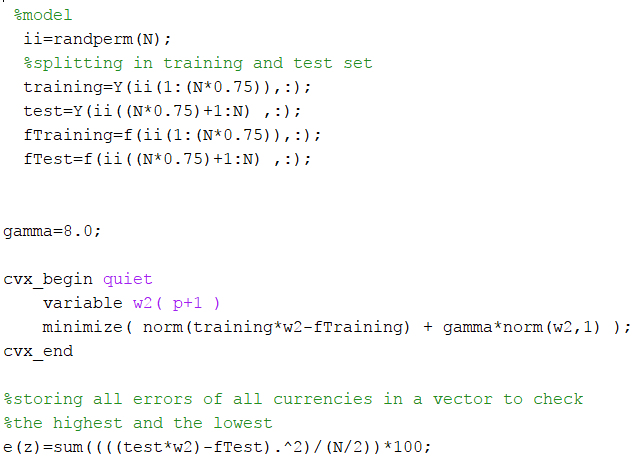
\includegraphics[width=0.4\textwidth]{error.png}

How is possible see in the application we put two tables containing the top 3 most and the top 3 least predictable exchange rates, the currencies exchanges with the lowest error and the highest error on the test set respectively.


\subsection{Justification}

At the beginning there were some doubts about using regression technique or an ANN(Artificial Neural network).
Both methods and merits and de-merits but at the end we chose to use linear regression principally for two reasons : 
\begin{itemize}
\item the main reason was that the ANN is a “black box” method and it is very difficult find any relationships between variables, on the contrary these relationships can easily be shown by regression models. 
\item the method of least squared regression converge much faster than a neural network, and this means a saving of resources and time 


\end{itemize}













\bibliographystyle{plain}
\bibliography{bib}

\end{document}